\documentclass[25pt]{sciposter}

\usepackage[T1]{fontenc}
\usepackage[utf8]{inputenc}

\usepackage{amsthm}

\usepackage[dvipsnames,usenames,svgnames,table]{xcolor} 
\usepackage{lipsum}
\usepackage{epsfig}
\usepackage{amsmath}
\usepackage{amssymb}
\usepackage[german]{babel}
\usepackage{geometry}
\usepackage{multicol}
\usepackage{graphicx}
\usepackage{tikz}
\usepackage{wrapfig}
\usepackage{gensymb}
\usepackage[utf8]{inputenc}
\usepackage{empheq}
\usepackage{mathtools}

\graphicspath{ {img/} }

\geometry{
 landscape,
 a1paper,
 left=5mm,
 right=50mm,
 top=5mm,
 bottom=50mm,
 }



%BEGIN LISTINGDEF



\usepackage{listings}
\usepackage{sourcecodepro}
\definecolor{listing-background}{rgb}{0.97,0.97,0.97}
\definecolor{listing-rule}{HTML}{B3B2B3}
\definecolor{listing-numbers}{HTML}{B3B2B3}
\definecolor{listing-text-color}{HTML}{000000}
\definecolor{listing-keyword}{HTML}{435489}
\definecolor{listing-identifier}{HTML}{435489}
\definecolor{listing-string}{HTML}{00999a}
\definecolor{listing-comment}{HTML}{8e8e8e}
\definecolor{listing-javadoc-comment}{HTML}{006CA9}

\lstdefinestyle{eisvogellistingstyle}{
	language=java,
	numbers=left,
	backgroundcolor=\color{listing-background},
	basicstyle=\color{listing-text-color}\small\ttfamily{}, % print whole listing small
	xleftmargin=0.8em, % 2.8 with line numbers
	breaklines=true,
	frame=single,
	framesep=0.6mm,
	rulecolor=\color{listing-rule},
	frameround=ffff,
	framexleftmargin=0.4em, % 2.4 with line numbers | 0.4 without them
	tabsize=4, %width of tabs
	numberstyle=\color{listing-numbers},
	aboveskip=1.0em,
	keywordstyle=\color{listing-keyword}\bfseries, % underlined bold black keywords
	classoffset=0,
	sensitive=true,
	identifierstyle=\color{listing-identifier}, % nothing happens
	commentstyle=\color{listing-comment}, % white comments
	morecomment=[s][\color{listing-javadoc-comment}]{/**}{*/},
	stringstyle=\color{listing-string}, % typewriter type for strings
	showstringspaces=false, % no special string spaces
	escapeinside={/*@}{@*/}, % for comments
	literate=
	{á}{{\'a}}1 {é}{{\'e}}1 {í}{{\'i}}1 {ó}{{\'o}}1 {ú}{{\'u}}1
	{Á}{{\'A}}1 {É}{{\'E}}1 {Í}{{\'I}}1 {Ó}{{\'O}}1 {Ú}{{\'U}}1
	{à}{{\`a}}1 {è}{{\'e}}1 {ì}{{\`i}}1 {ò}{{\`o}}1 {ù}{{\`u}}1
	{À}{{\`A}}1 {È}{{\'E}}1 {Ì}{{\`I}}1 {Ò}{{\`O}}1 {Ù}{{\`U}}1
	{ä}{{\"a}}1 {ë}{{\"e}}1 {ï}{{\"i}}1 {ö}{{\"o}}1 {ü}{{\"u}}1
	{Ä}{{\"A}}1 {Ë}{{\"E}}1 {Ï}{{\"I}}1 {Ö}{{\"O}}1 {Ü}{{\"U}}1
	{â}{{\^a}}1 {ê}{{\^e}}1 {î}{{\^i}}1 {ô}{{\^o}}1 {û}{{\^u}}1
	{Â}{{\^A}}1 {Ê}{{\^E}}1 {Î}{{\^I}}1 {Ô}{{\^O}}1 {Û}{{\^U}}1
	{œ}{{\oe}}1 {Œ}{{\OE}}1 {æ}{{\ae}}1 {Æ}{{\AE}}1 {ß}{{\ss}}1
	{ç}{{\c c}}1 {Ç}{{\c C}}1 {ø}{{\o}}1 {å}{{\r a}}1 {Å}{{\r A}}1
	{€}{{\EUR}}1 {£}{{\pounds}}1 {«}{{\guillemotleft}}1
	{»}{{\guillemotright}}1 {ñ}{{\~n}}1 {Ñ}{{\~N}}1 {¿}{{?`}}1
}
\lstset{style=eisvogellistingstyle}



%END LISTINGDEF


\newcommand*\widefbox[1]{\fbox{\hspace{2em}#1\hspace{2em}}}


\newlength\dlf  % Define a new measure, dlf
\newcommand\alignedbox[2]{
% Argument #1 = before & if there were no box (lhs)
% Argument #2 = after & if there were no box (rhs)
&  % Alignment sign of the line
{
\settowidth\dlf{$\displaystyle #1$}
    % The width of \dlf is the width of the lhs, with a displaystyle font
\addtolength\dlf{\fboxsep+\fboxrule}
    % Add to it the distance to the box, and the width of the line of the box
\hspace{-\dlf}
    % Move everything dlf units to the left, so that & #1 #2 is aligned under #1 & #2
\boxed{#1 #2}
    % Put a box around lhs and rhs
}
}
\usepackage{graphicx,url}

%BEGIN TITLE
\title{\huge{Analysis 1}}

\author{\large{David Zollikofer}}
%END TITLE

\usepackage{palatino}

% begin custom commands
\newcommand{\Q}{\mathbb{Q}}
\newcommand{\R}{\mathbb{R}}
\newcommand{\N}{\mathbb{N}}



\newtheorem{thm}{Thm}[section]



\usepackage[framemethod=TikZ]{mdframed}
\newenvironment{method}[1]{\begin{mdframed}[backgroundcolor=blue!10,innertopmargin=15pt, innerbottommargin=15pt]
		\textbf{#1 }
	}
	{ 
	\end{mdframed}
}
\usepackage{todonotes}
\newcommand{\TODO}[1]{\todo[inline]{\Large TODO:  #1}}


\DeclarePairedDelimiter\abs{\left|}{\right|}%
\DeclarePairedDelimiter\norm{\lVert}{\rVert}%
% end custom commands

\begin{document}

\fontfamily{ppl}\selectfont



\maketitle


\begin{multicols}{3}


\section{Einführung}

\subsection{Ordnungsvollständigkeit}
Unterscheidet $\R$ von $\Q$. Für $A,B$ nichtleere Teilmengen von $\R$ mit $$\forall a\in A \land \forall b \in B \implies a \leq b$$
Dann gibt es $c \in \R$ mit $\forall a \in A : a \leq c$ und $\forall b \in B : c \leq b$

\subsection{Archimedisches Prinzip}
Korollar von Ordnungsvollständigkeit. Sei $x\in \R$ mit $x>0$ und $y \in \R$, dann gibt es $n\in \N$ mit $y \leq nx$

\subsection{Youngsche Ungleichung}
$\forall \epsilon > 0 , \forall x,y\in \R$ gilt: $2 |xy| \leq \epsilon x^2 + \frac{1}{\epsilon} y^2$. Beweis per Expansion von $\left( \sqrt{\epsilon} |x| - \frac{1}{\sqrt{\epsilon}} |y| \right) ^2 \geq 0$

\subsection{Existenz des Supremums}
Sei $A \subset \R$, $A \not = \varnothing$. Sei $A$ nach oben beschränkt, dann gibt es eine kleinste obere Schranke von $A$, $c = \sup A$, genannt Supremum von $A$. Um dies zu Beweisen nutzt man die Ordnungsvollständigkeit und definiert $B$ als die Menge der oberen Schranken.

\subsection{Cauchy Schwarz}
$\forall x,y\in \R^n$ gilt $|\langle x,y\rangle| \leq ||x||\cdot||y||$.

\subsection{Komplexe Zahlen}
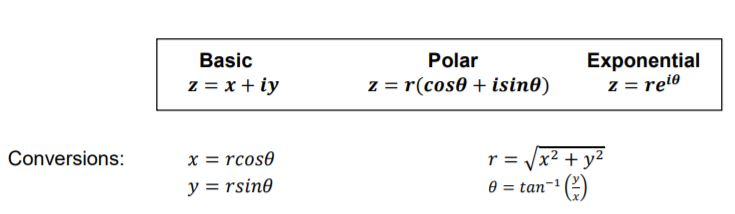
\includegraphics[scale=1.4]{complex.jpg}\\
\textsc{Division:} Es gilt $z^{-1} = \frac{\bar{z}}{||z||^2}$ wenn $z \not = 0$\\
\textsc{Polarform} Wenn \begin{align*}
z_1 &= r_1(\cos(\theta_1) + i\sin(\theta_1))\\
z_2 &= r_2(\cos(\theta_2) + i\sin(\theta_2))
\end{align*}
dann gilt: 
\begin{align*}
z_1 \cdot z_2 &= r_1 \cdot r_2 \left(\cos(\theta_1 + \theta_2) + i\sin(\theta_1 + \theta_2)\right)\\
\frac{z_1}{z_2} &= \frac{r_1}{r_2}\left(\cos(\theta_1 - \theta_2) + i\sin(\theta_1 - \theta_2)\right)
\end{align*}
Zudem folgt durch Induktion:
$$z^n = r^n (\cos(n\theta) + i \sin(n \theta))$$




\newpage


% -------------------------- Folgen --------------------------

\section{Folgen}

\TODO{ add defs of convergence and divergence}
\TODO{Beweis mittels definition}

\begin{method}{Rechnen mit Grenzwerten} $(a_n)_n$ und $(b_n)_n$ konvergent mit GW $a,b$. Dann gilt:
	\begin{itemize}
		\item $\lim \limits_{n \to \infty} (a_n + b_n) = a + b$	
		\item $\lim \limits_{n \to \infty} (a_n \cdot b_n) = a \cdot b$
		\item  Falls $b_n, b \not = 0$, so gilt $\lim \limits_{n \to \infty} \frac{a_n}{b_n} = \frac{a}{b}$
		\item Falls $a_n \leq b_n$ $\forall n \in \mathbb{N}$, so gilt $a \leq b$
	\end{itemize}
\end{method}

\TODO{Bsp p 69 ff.}


\begin{method}{Sandwich Theorem}
Seien $b_n \leq a_n \leq c_n$. Falls $b_n$ und $c_n$ konvergent sind mit $\lim \limits_{n \to \infty } b_n = \lim \limits_{n \to \infty } c_n = L$, so ist $a_n$ auch konv. mit $\lim \limits_{n \to \infty } a_n = L$
\end{method}
\TODO{add proof sandwich}
\TODO{add examples}
% -------------------------- Reihen --------------------------

\section{Reihen}
\begin{method}{Konvergenz mit Definition} Eine Reihe konvergiert wenn der Grenzwert der Partialsummen existiert:
	$$\sum_{n=0}^{\infty} a_n  = \lim\limits_{N\to\infty} S_n = \lim\limits_{N\to\infty} \sum_{n=0}^{\infty} a_n$$
\end{method}
\TODO{Bsp fehlt}
\begin{method}{Konvergenz mit $\lim\limits_{n \to \infty } a_n = 0$}
$$\sum_{n=0}^{\infty} a_0 \text{ konvergiert } \implies \lim\limits_{n \to \infty } a_n = 0 $$
\end{method}
\TODO{Bsp fehlt}


\begin{method}{Majorantenkriterium}
	Fall $a_n \geq b_n \forall n \geq n_0$ für ein $n_0$. Dann gilt $\sum_n a_n \text{ konvergiert } \implies \sum_{n} b_n$ konvergiert.
\end{method}

\begin{method}{Minorantenkriterium}
	Fall $a_n \geq b_n \forall n \geq n_0$ für ein $n_0$. Dann gilt $\sum_n b_n \text{ divergiert } \implies \sum_{n} a_n$ divergiert.
\end{method}




\begin{method}{Quotientenkriterium}
	Sei $a_n \not = 0$, dann gilt:
	\begin{itemize}
		\item $\lim\limits_{n \to \infty} |\frac{a_{n+1}}{a_n}|> 1 \implies \sum_{n} a_n$ divergiert. 
		\item $\lim\limits_{n \to \infty} |\frac{a_{n+1}}{a_n}|< 1 \implies \sum_{n} a_n$ konvergiert. 
		\item $\lim\limits_{n \to \infty} |\frac{a_{n+1}}{a_n}|=  1 \implies $ Kriterium versagt.
	\end{itemize}
\end{method}
\TODO{Beispiel \& Beweis}





\begin{method}{Wurzelkriterium}
	\begin{itemize}
		\item $\lim\limits_{n \to \infty} \sqrt[n]{|a_n|}>1 \implies \sum_{n} a_n $ divergiert
		\item $\lim\limits_{n \to \infty} \sqrt[n]{|a_n|}<1 \implies \sum_{n} a_n $ konvergiert
		\item $\lim\limits_{n \to \infty} \sqrt[n]{|a_n|}=1 \implies $ Kriterium versagt
	\end{itemize}
\end{method}

\TODO{Beispiel \& BEweis}



\begin{method}{Integralkriterium} Wenn $\sum_{n=p}^{\infty} a_n$ sowohl $a_n \geq 0$ und $a_{n+1} \leq a_n$ (monot. fall.), dann gilt:
$$\sum_{n=p}^{\infty} a_n \text{ konv. } \iff \int_{p}^{\infty} a(x) dx \text{ konv.}$$
\end{method}
\TODO{Frage ob legal}


\begin{method}{Leibnitzkriterium} Eine Reihe $\sum_n (-1)^n a_n$ konvergiert falls $a_n \geq 0$ , $\lim\limits_{n \to \infty } a_n = 0$ und $a_n$ monoton fallend ist.
\end{method}

\textbf{Beispiel (Leibnitz)}: $\sum_{n = 1}^{\infty} \frac{\cos(2\pi n)}{\cos(n \pi)} \frac{\log(n)}{n^2}$. Wir stellen fest dass $\sum_{n = 1}^{\infty} \frac{\cos(2\pi n)}{\cos(n \pi)} \frac{\log(n)}{n^2} = \sum_{n = 1}^{\infty} (-1)^n \frac{\log(n)}{n^2}$. Zudem gilt $\frac{\log(n)}{n^2} \geq 0$, sowie $\lim\limits_{n \to \infty} \frac{\log(n)}{n^2} = 0$. Zudem ist $\frac{\log(n)}{n^2}$ monot. fallend für $n \geq 2$, da: 
$$ \frac{d}{dx} \frac{\log(x)}{x^2} = -2 \frac{\log(x)}{x^3} + \frac{1}{x} = \frac{1- 2\log(x)}{x^3} \leq 0\text{ } \forall x \geq \sqrt{e} = 1.6..$$





\begin{method}{Absolute Konvergent}
	Eine Reihe $\sum_{n} a_n$ ist absolut konvergent falls $\sum_{n} |a_n|$ konvergiert.
\end{method}

\textbf{Beispiel (Absolute Konvergenz)} Ang. $\sum_{n} a_n$ konvergiert absolut. Betrachte $\sum_{n=0}^{\infty} (\sqrt{1 + a_n} -1)$ und bemerke dass es auch abs. konv.
$$\left|\sqrt{1 + a_n} -1\right| = \left| (\sqrt{1 + a_n} -1) \frac{\sqrt{1 + a_n} +1}{\sqrt{1 + a_n} +1} \right| = \left| \frac{a_n}{\sqrt{1 + a_n} + 1} \right| \leq |a_n|$$

\TODO{Sätze aus dem Skript zur absoluten Konvergenz}




\newpage

\end{multicols}
\end{document}